\section{Implementation Details}

\subsection{Implementation Successes}
We found that the general flowchart (see Figure \ref{fig:data_flow}) we had designed for implementing the software library was accurate. Hence, during each work session, we were able to identify modules of the Raft consensus algorithm from our flowchart and successfully implement these modules using the API exposed to us by the painlessMesh software library, updating our understanding along the way. The following is a list of our successes in attempting to implement Raft atop painlessMesh:

\begin{itemize}
  \item Designing a UML diagram (see Figure \ref{fig:uml}) to document and build a detailed architecture of our software library.
  \item Setting up a PlatformIO (PIO) project capable of uploading and managing the ESP devices being tested. This PIO project will also for eventual end-users to rapidly install and work with our software library.
  \item Implementing a virtual testing framework (see Figure \ref{fig:virtual_ramen}) that mimics painlessMesh and interacts with our library to simulate a large number of nodes for debugging and scale-testing purposes.
  \item Completing the initialization, voting communication, state switching, and leader selection modules of the Raft consensus algorithm.
  \item Designing a portable PCB (as specified in Figure \ref{fig:final_design_prototype}) with an ESP8266 chip, various sensors, an on-board battery case that will allow us to conduct scale and distance tests for our software library. The completed schematic and PCB designs can be seen in Figures \ref{fig:pcb_schematic} and \ref{fig:pcb}.
\end{itemize}

\subsection{Issues Faced}
We did not come across any significant challenges when building our software library. The notable challenges we came across were a result of a mismatch between our flowchart and UML diagram against the Raft paper \cite{raft_paper}. Hence, throughout our implementation sessions, we returned back to the Raft consensus algorithm and better understood the details so that we could accurately implement these details in our software library. This involved us updating the flowchart and UML diagram to align with the framework outlined in the Raft consensus algorithm paper.r

Every bug we encountered involving unexpected behavior was quickly identified by referencing our log messages and finding anomalies in our virtual testing framework. Then, the fixed behavior was compared against the interactive browser implementation of Raft \cite{raft_webiste} to ensure accurate implementation. 

\subsection{Changes Made}
The Raft consensus algorithm accounts for multiple clients on the network attempting to pass data onto the servers. Specifically, the Raft paper states that "if a client contacts a follower, the follower redirects it to the leader" \cite{raft_paper}. However, this situation assumes a network where clients have direct access to the leader. In the case of a network of embedded devices, we consider the "clients" to be the sensors on each node. Hence, these "clients" do not have direct access to the leader. As a result, we slightly modify the Raft algorithm to account for such scenarios. 

We envision each follower node to have a client associated with it. In our suggested modification, these clients, when seeking to add data to the network's logs, are not redirected to the network's leader node. Rather, they add their data to the server's data buffer. At each time interval, the follower node checks its data buffer to forward these messages to the leader node's data buffer. Similarly, the leader node periodically checks its data buffer for such messages, which are then pushed into the network using the Raft algorithm. 

Our modification remains true to the operation of the Raft consensus algorithm in that follower nodes are not allowed to push data into the network. We simply provide an alternative implementation given that most clients on the network cannot directly access the leader node. 

\subsection{Initial Results}
As we have mentioned earlier, we created a virtual testing framework for our software library. The framework is capable of creating hundreds of virtual boards for testing our code. In real life, it wouldn't be possible to test our software at this scale both due to budget and time constraints. It takes about 30 seconds to compile and upload to each board. We also don't have that many boards. Thus, the virtual testing framework lets us rapidly test our code and debug where needed.

Figure \ref{fig:virtual_ramen} shows a virtual network of 3 nodes running the initial version of our software library. When we look at the log messages outputted by each node, we see that node 1 starts an election and requests votes from the other nodes. Later, nodes 2 and 3 grants vote to node 1 during the election. 

\begin{figure}[H]
    \centering
    \subfloat{{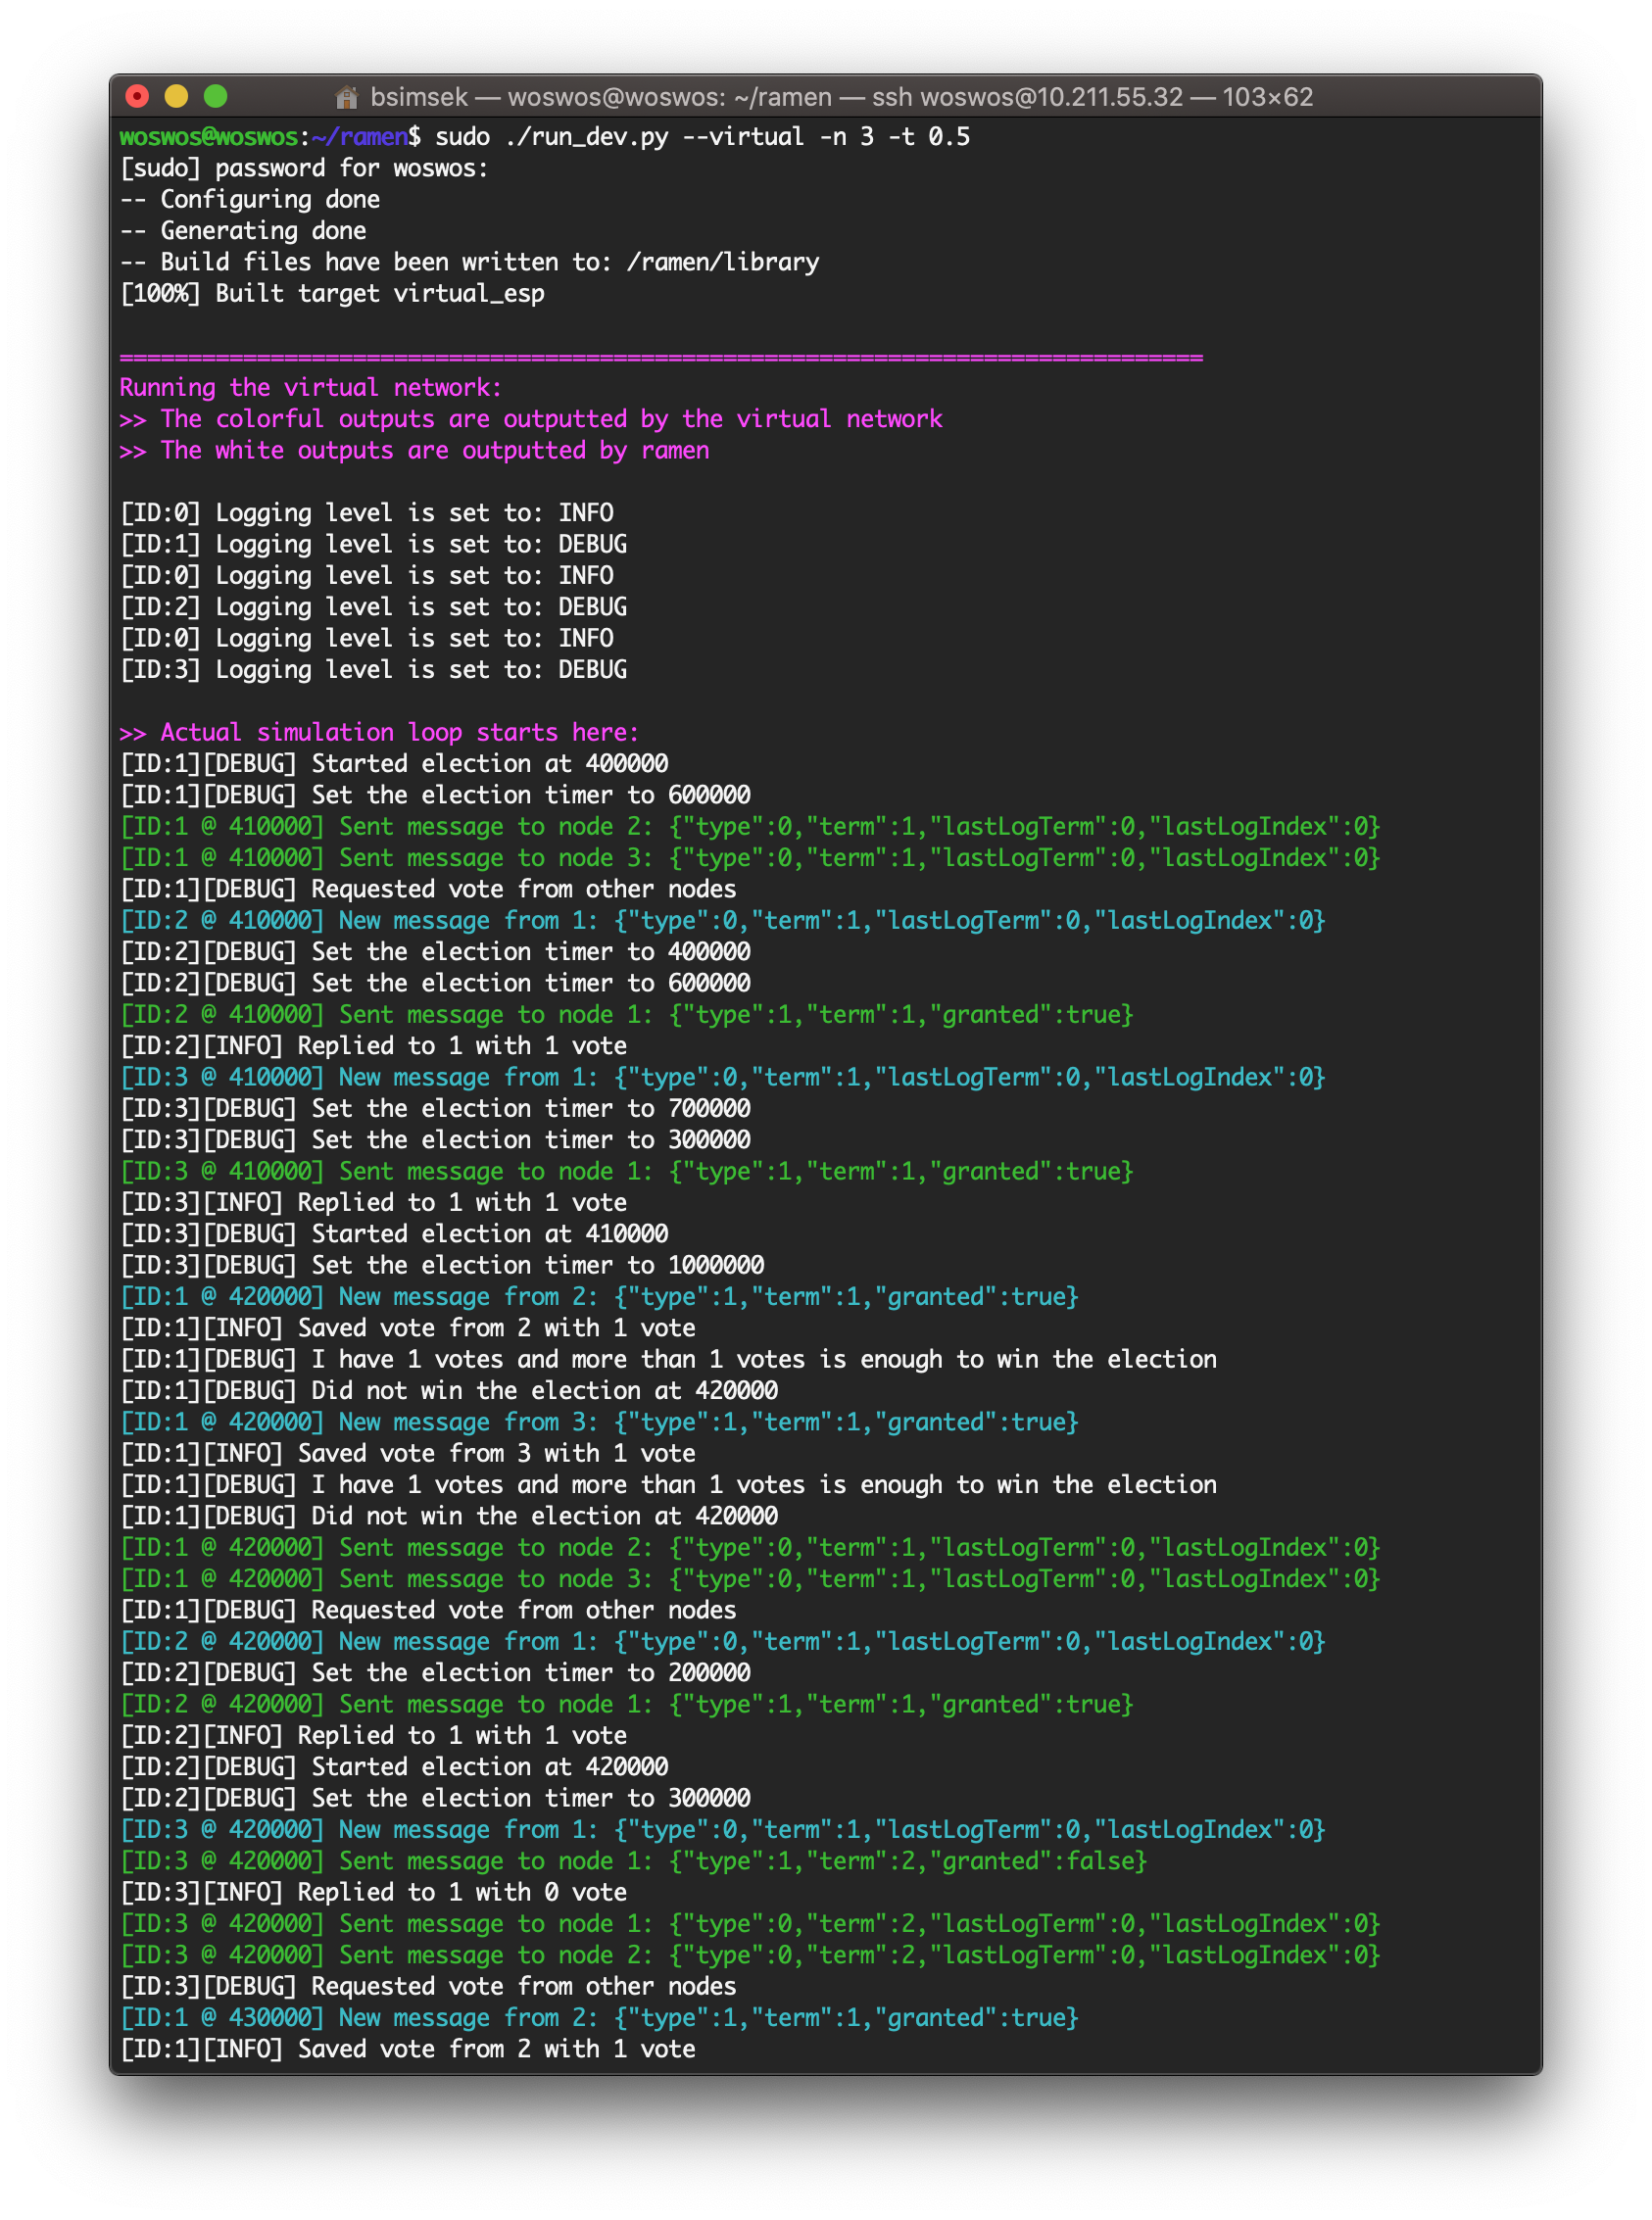
\includegraphics[width=0.46\columnwidth]{images/virtual_ramen_1.png} }}%
    \qquad
    \subfloat{{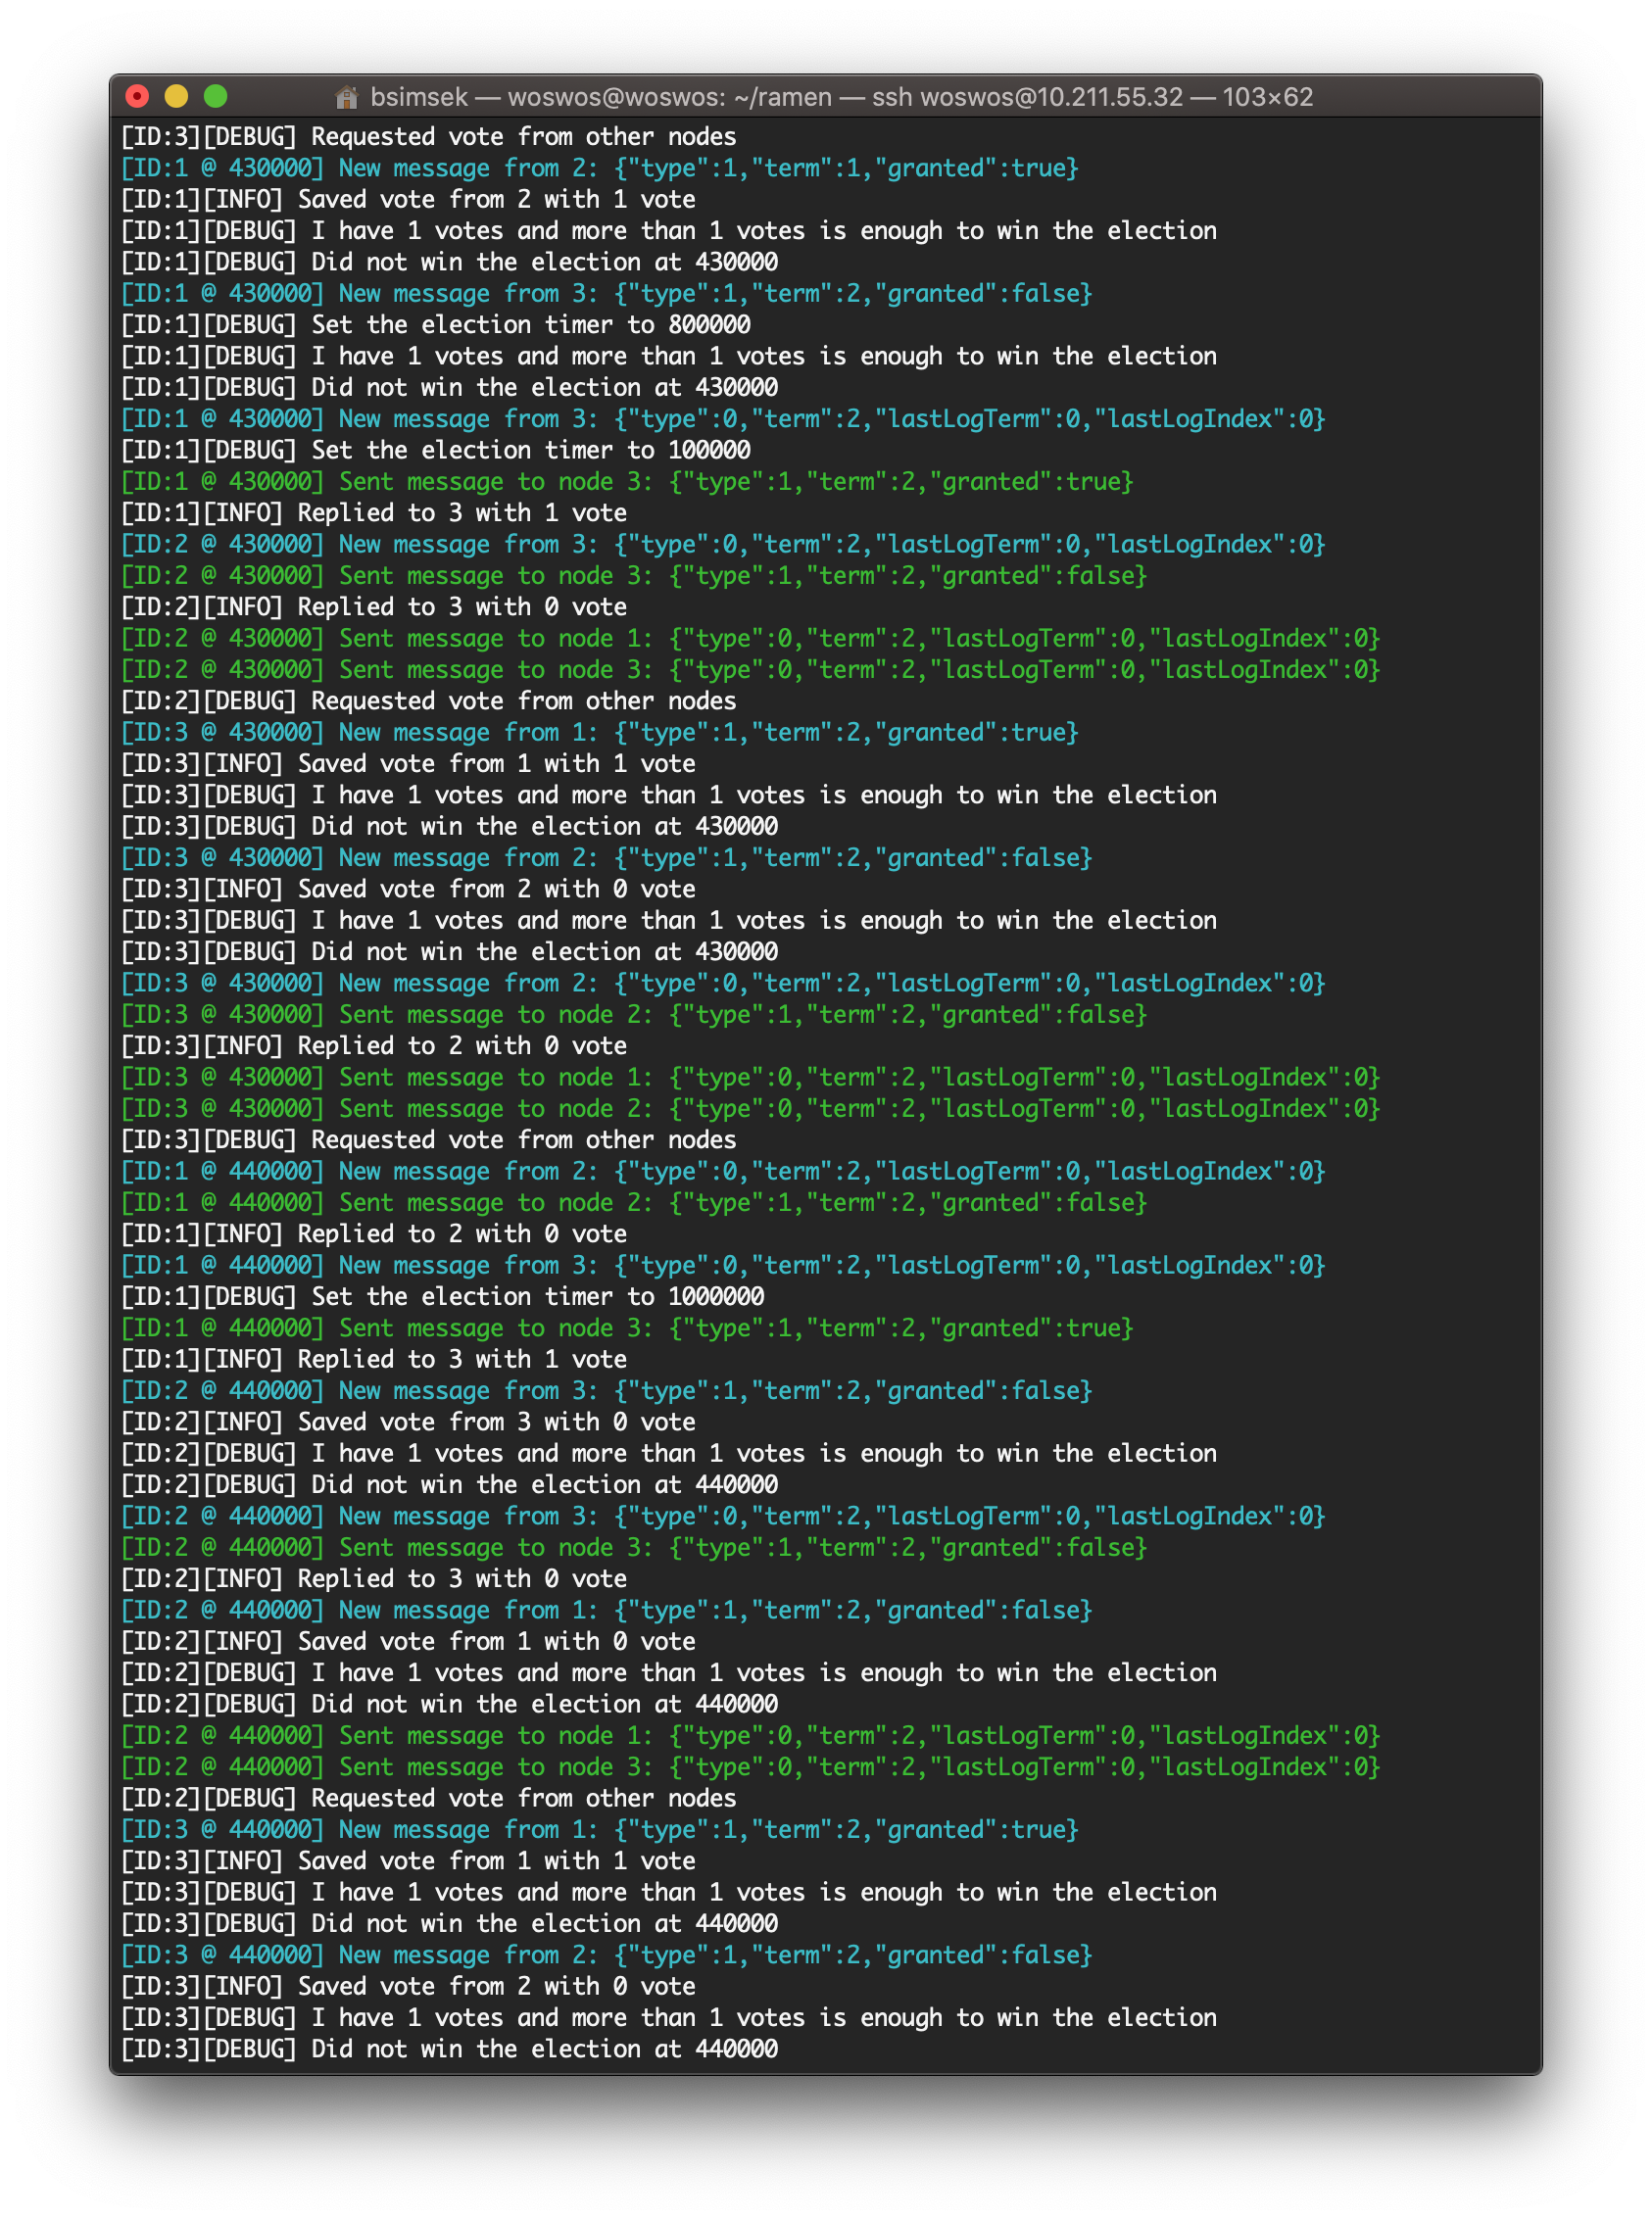
\includegraphics[width=0.46\columnwidth]{images/virtual_ramen_2.png}}}%
    \caption{ramen software running in the virtual simulated mesh network environment. The window on the left shows the beginning of the simulation and the windows on the right shows the remaining parts of the simulation}
    \label{fig:virtual_ramen}%
    \medskip
\end{figure}

In addition to the virtual testing framework, we also tested the initial version on the physical boards we have and confirmed the functionality. However, having the virtual testing beforehand lets us save a lot of development time.